% LaTeX document: Rationale and Performance of Chain Reaction Heuristics
\documentclass[12pt]{article}
\usepackage[utf8]{inputenc}
\usepackage[T1]{fontenc}
\usepackage{lmodern}
\usepackage{geometry}
\geometry{margin=1in}
\usepackage{booktabs}
\usepackage{graphicx}
\usepackage{subcaption}

\title{Heuristics in Chain Reaction AI Agent}
\author{Nafis Nahian | ID : 2105007} 
\date{16 June 2025}

\begin{document}

\maketitle
\vspace{1em}

\section{Experimental Setup}

This report analyzes the performance of six different heuristic functions implemented for the
 Chain Reaction AI player. Each heuristic was tested at search \textbf{depths 2-4}, measuring the average
 time taken to complete 3 games with other AI agents. For faster evaluation, the results were calculated by running
 on a \textbf{5x5 grid} with \textbf{10 sec time limit} per move for an AI agent. 

\section{Heuristic Rationale}

\subsection{Orb-Count Heuristic}
The orb-count heuristic measures the simple difference in total orbs between the current player and their opponent. This metric serves as a baseline evaluation of material advantage. A higher orb count typically indicates greater board control and available resources for creating chain reactions. Due to its low computational cost, it provides an efficient first approximation of the game state.

\subsection{Explosion Potential Heuristic}
The explosion potential heuristic evaluates the immediate tactical opportunities on the board. It:
\begin{itemize}
  \item Rewards cells that are one orb shy of exploding, as these can trigger chain reactions on the next move.
  \item Adds bonus points when a nearly critical cell is adjacent to an opponent's cell, representing an "attack" opportunity to capture or disrupt enemy cells.
  \item Accounts for supporting neighbors of the same player, reflecting local buildup that can feed into larger explosions.
  \item Penalizes opponent cells that are about to explode, encouraging moves that avoid handing free chain reactions to the opponent.
\end{itemize}
This heuristic focuses on short-term burst potential rather than long-term positioning.

\subsection{Strategic-Evaluation Heuristic}
The strategic-evaluation heuristic blends material, positional, and threat-aware considerations. Key components include:
\begin{itemize}
  \item \textbf{Orb count contribution:} Adds total orbs owned to reinforce material advantage.
  \item \textbf{Positional bonuses:} Corners receive a higher bonus for safety (fewer overflow directions), and edges receive a moderate bonus, reflecting more controlled risk.
  \item \textbf{Explosive readiness:} Rewards cells at critical-1 for future chain opportunities.
  \item \textbf{Opponent threat mitigation:} Applies penalties when opponent cells adjacent to yours are about to explode, highlighting urgent defensive needs.
\end{itemize}
By combining these factors, this heuristic guides mid-game planning and board shaping.

\subsection{Threat-Analysis Heuristic}
The threat-analysis heuristic is designed for advanced defense and risk assessment:
\begin{itemize}
  \item \textbf{Immediate threats:} Detects opponent cells that will explode on their next turn. If you cannot counter that by exploding a neighboring cell in the next move (can not block), a larger penalty is applied.
  \item \textbf{Potential threats:} Flags cells two orbs away from critical, scaling penalties by how close they are to exploding.
  \item \textbf{Defensive formations:} Rewards clusters of your own cells that reinforce each other, encouraging solid defensive walls.
  \item \textbf{Global assessment:} Normalizes the count of immediate and potential threats by board size, applying a heavy penalty to overall vulnerability.
\end{itemize}
This heuristic prioritizes risk mitigation and encourages moves that reduce opponent threat levels.

\subsection{Tempo Heuristic}
The tempo heuristic measures initiative and move-forcing capability:
\begin{itemize}
  \item \textbf{Forcing moves:} Counts cells at critical-2 for both players—these moves pressure opponents by creating imminent explosions.
  \item \textbf{Development ratio:} Compares total orb counts to determine who is leading in board growth.
  \item \textbf{Initiative score:} Combines forcing move differences to reflect which player is dictating the pace of play.
\end{itemize}
By valuing positions that force immediate responses, this heuristic captures control over the game's tempo.

\subsection{Strategic Eval + Explosion Potential Combined Heuristic}
This combined heuristic integrates long-term positional strength of Strategic-Evaluation Heuristic with short-term tactical opportunities from Explosion Potential Heuristic. It doubles the strategic-evaluation score to emphasize board shape and adds the explosion potential score to keep chain reaction bursts on the radar. The result is a balanced evaluation that neither over-prioritizes local combos nor neglects overall positioning.

\section{Performance Evaluation}

For each depth, Table 1,2 and 3 summarizes average move time, win rate, and average moves per depth. Figures illustrate move times and win rates.

% Depth 2
\subsection{Depth 2 Performance}
\begin{table}[ht]
  \centering
  \caption{Performance Metrics at Depth 2}
  \label{tab:metrics_depth2}
  \begin{tabular}{lccc}
    \toprule
    Heuristic                & Avg Move Time (s) & Win Rate (\%) & Avg Moves \\
    \midrule
    Orb Count                & 0.0049            & 26.67         & 51.7      \\
    Explosion Potential      & 0.0065            & 60.00         & 54.7      \\
    Strategic Evaluation     & 0.0060            & 40.00         & 52.8      \\
    Threat Analysis          & 0.0089            & 23.33         & 52.4      \\
    Tempo                    & 0.0058            &  0.00         & 43.4      \\
    Combined Heuristic       & 0.0076            & 46.67         & 53.8      \\
    \bottomrule
  \end{tabular}
\end{table}

% \begin{figure}[ht]
%   \centering
%   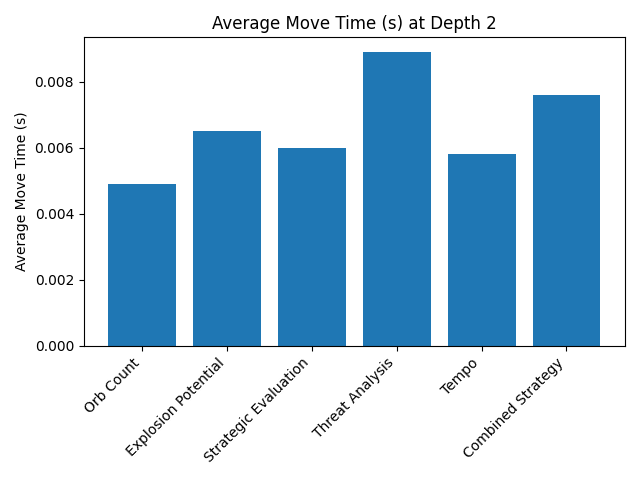
\includegraphics[width=0.7\textwidth]{depth2_move_time.png}
%   \caption{Average move time at depth 2}
%   \label{fig:move2}
% \end{figure}

% \begin{figure}[ht]
%   \centering
%   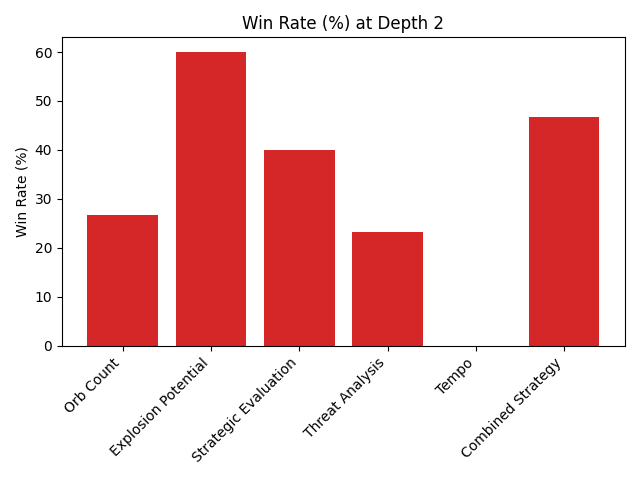
\includegraphics[width=0.7\textwidth]{depth2_win_rate.png}
%   \caption{Win rates at depth 2}
%   \label{fig:win2}
% \end{figure}

\begin{figure}[ht]
  \centering
  \begin{subfigure}[b]{0.45\textwidth}
    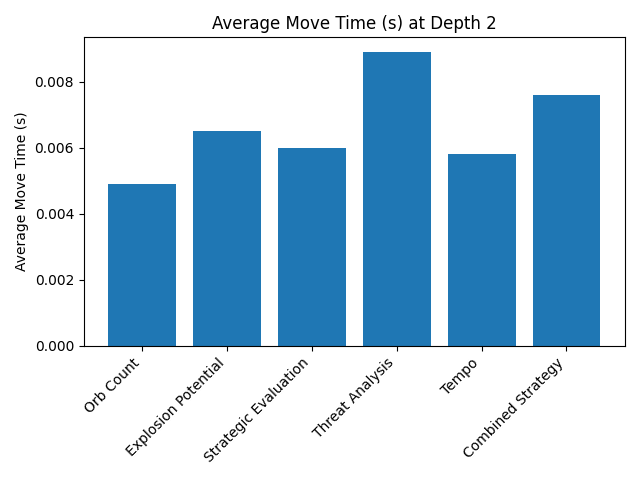
\includegraphics[width=\textwidth]{depth2_move_time.png}
    \caption{Avg Move Time at Depth 2}
    \label{fig:move2}
  \end{subfigure}
  \hfill
  \begin{subfigure}[b]{0.45\textwidth}
    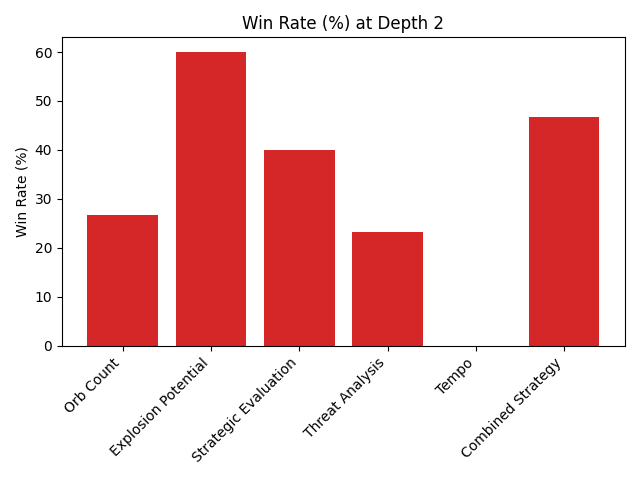
\includegraphics[width=\textwidth]{depth2_win_rate.png}
    \caption{Win Rate at Depth 2}
    \label{fig:win2}
  \end{subfigure}
  \caption{Performance metrics for heuristics at depth 2}
  \label{fig:perf2}
\end{figure}


% Depth 3
\subsection{Depth 3 Performance}
\begin{table}[ht]
  \centering
  \caption{Performance Metrics at Depth 3}
  \label{tab:metrics_depth3}
  \begin{tabular}{lccc}
    \toprule
    Heuristic                & Avg Move Time (s) & Win Rate (\%) & Avg Moves \\
    \midrule
    Orb Count                & 0.0447            & 46.67         & 53.2      \\
    Explosion Potential      & 0.0635            & 53.33         & 54.0      \\
    Strategic Evaluation     & 0.0742            & 86.67         & 52.9      \\
    Threat Analysis          & 0.0619            & 50.00         & 49.7      \\
    Tempo                    & 0.0279            & 10.00         & 45.7      \\
    Combined Heuristic       & 0.0915            & 80.00         & 52.3      \\
    \bottomrule
  \end{tabular}
\end{table}

\begin{figure}[ht]
  \centering
  \begin{subfigure}[b]{0.45\textwidth}
    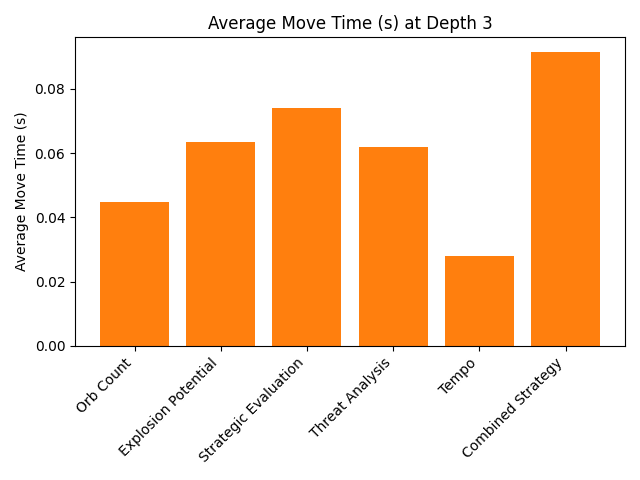
\includegraphics[width=\textwidth]{depth3_move_time.png}
    \caption{Avg Move Time at Depth 2}
    \label{fig:move2}
  \end{subfigure}
  \hfill
  \begin{subfigure}[b]{0.45\textwidth}
    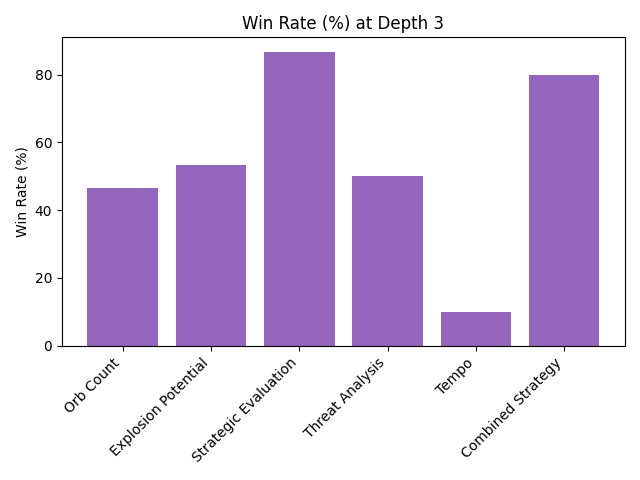
\includegraphics[width=\textwidth]{depth3_win_rate.png}
    \caption{Win Rate at Depth 2}
    \label{fig:win2}
  \end{subfigure}
  \caption{Performance metrics for heuristics at depth 2}
  \label{fig:perf2}
\end{figure}

% Depth 4
\newpage
\subsection{Depth 4 Performance}
\begin{table}[h!]
  \centering
  \caption{Performance Metrics at Depth 4}
  \label{tab:metrics_depth4}
  \begin{tabular}{lccc}
    \toprule
    Heuristic                & Avg Move Time (s) & Win Rate (\%) & Avg Moves \\
    \midrule
    Orb Count                & 0.1939            & 66.67         & 59.0      \\
    Explosion Potential      & 0.2884            & 86.67         & 51.4      \\
    Strategic Evaluation     & 0.2521            & 56.67         & 58.6      \\
    Threat Analysis          & 0.3698            & 73.33         & 58.0      \\
    Tempo                    & 0.1621            &  6.67         & 43.0      \\
    Combined Heuristic       & 0.2865            & 86.67         & 54.6      \\
    \bottomrule
  \end{tabular}
\end{table}

\begin{figure}[ht]
  \centering
  \begin{subfigure}[b]{0.45\textwidth}
    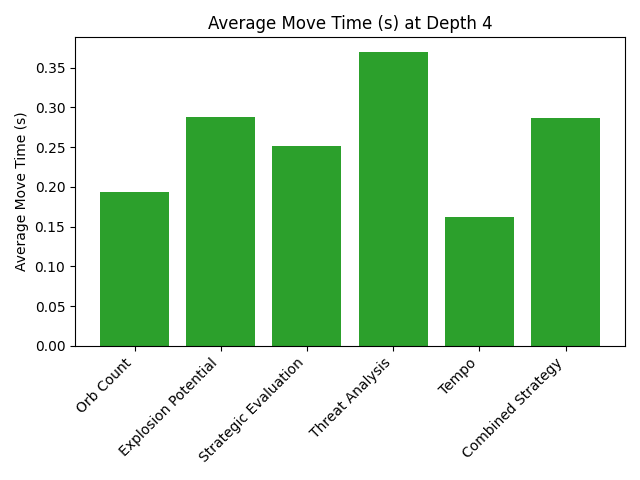
\includegraphics[width=\textwidth]{depth4_move_time.png}
    \caption{Avg Move Time at Depth 2}
    \label{fig:move2}
  \end{subfigure}
  \hfill
  \begin{subfigure}[b]{0.45\textwidth}
    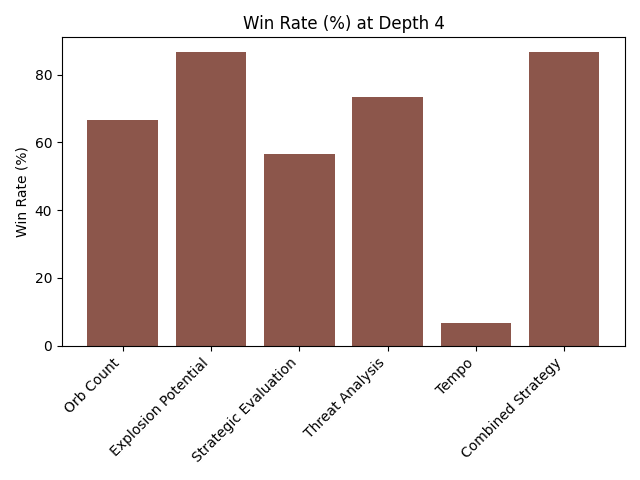
\includegraphics[width=\textwidth]{depth4_win_rate.png}
    \caption{Win Rate at Depth 2}
    \label{fig:win2}
  \end{subfigure}
  \caption{Performance metrics for heuristics at depth 2}
  \label{fig:perf2}
\end{figure}

\newpage
\section{Overall Comparison and Recommendations}
Analyzing both efficiency and effectiveness:
\begin{itemize}
  \item \textbf{Depth 2:} Orb Count offers the fastest response but low win rate. On the other hand Explosion Potential provides balanced move time and Highest win percentage.
  \item \textbf{Depth 3:} Combined Heuristic and Strategic Evaluation reach high win rates (~80--87\%) at moderate times (<0.1s), making depth 3 a strong choice. 
    Differing from depth 2, Tempo responses the fastest in depth 3 instead of Orb Count, but it has the lowest win rate.
  \item \textbf{Depth 4:} Consistent with depth 3, Tempo has both the lowest Average move time and win rate. 
  Highest win rates appear for both Explosion Potential and Combined Heuristic (~86\%), but move times exceed 0.28s—only suitable when latency is less critical.
  \item \textbf{If speed is a Priority:} Tempo and Orb Count remain lightweight but offer lower win rates; good for extremely time-sensitive scenarios.
  \item \textbf{If performance is a Priority:} Strategic Evaluation or Combined Heuristic at depth 4 provide the highest win rates around 87\%
  \item \textbf{For balanced play:} Depth 3 with Strategic Evaluation offers the best balance between speed and win rate, achieving over 80\% win rates under 0.1s.
\end{itemize}

\end{document}